\documentclass{article}
\usepackage{multirow}
\usepackage{subcaption}
\usepackage[utf8x]{inputenc} 
\usepackage{graphicx}
\usepackage{amssymb}
\usepackage{amsmath}
\usepackage{bm}
\usepackage{physics}
\usepackage{cite}
\usepackage{titlesec}
\usepackage{setspace}
\usepackage[margin=1.0in]{geometry}
%For numbering%%%
\usepackage{etoolbox}
\makeatletter
\patchcmd{\ttlh@hang}{\parindent\z@}{\parindent\z@\leavevmode}{}{}
\patchcmd{\ttlh@hang}{\noindent}{}{}{}
\makeatother
%%%%%%%%%%%%%%%%%
\title{PH4477 Assessed Practical Coursework}
\author{Michael Hayes}
\titleformat{\section}[block]
  {\fontsize{17.28}{18}\bfseries\sffamily\filcenter\raggedright}
  {\thesection}
  {1em}
  {}
\titleformat{\subsection}[hang]
  {\fontsize{14}{15}\bfseries\sffamily\filcenter\raggedright}
  {\thesubsection}
  {1em}
  {}
\titleformat{\subsubsection}[hang]
  {\fontsize{12}{14}\bfseries\sffamily\filcenter\raggedright}
  {\thesubsubsection}
  {1em}
  {}


\begin{document}
\maketitle
\large
\onehalfspacing

\section{Introduction}

The aim of this practical was to extend the functionality of a molecular dynamics program, written in python, named `pymold'. This extended version was then used to simulate a binary mixture of argon and krypton under similar conditions to the paper `Structure and diffusion in mixtures of rare-gas liquids' by G. Jacucci and I.R. McDonald 

\section{Pymold}
The project was based around a preexisting molecular dynamics program, that simulated the interactions between atoms in a system, tracking their positions as they varied through time. The program, written in Python \cite{TODO}, performed a number of calculations on the


\subsection{Extension to Pymold}


\subsubsection{Binary Mixtures}
Pymold was first extended to perform molecular dynamics simulations on binary mixtures of Lennard-Jones atoms. As these atoms may have different Lennard-Jones parameters, the effective values of $\sigma$ and $\epsilon$ when evaluating the LJ function are given by the Lorentz-Berthelot mixing rules

\begin{equation}
\sigma_{ij} = \frac{\sigma_{ii} + \sigma_{jj}}{2},
\end{equation}

and

\begin{equation}
\epsilon_{ij} = \sqrt{\epsilon_{ii}\epsilon{jj}}.
\end{equation}

The parameters for argon and krypton are shown in Table \ref{table:LJParams}.

\begin{table}[h!t]
\centering
\caption{The Lennard-Jones parameters for argon and krypton. The masses, and values for $\sigma$ and $\epsilon/k_{\rm{B}}$, are listed in \cite{ReviewOfParticlePhysics} and \cite{StructureAndDiffusion} respectively. \label{table:LJParams} }
\begin{tabular}{|c|c|c|c| } 
\hline
Element & Mass (Au)& $\sigma\,(\rm{\r{A}})$ & $\epsilon/k_{\rm{B}}\,$(K)\\\hline
Argon	& $39.948$ & $119.8$ & $3.405$ \\
Krypton	& $83.798$ & $167.0$ & $3.633$ \\
%Neon	& $20.1797$ & $36.2$ & $2.800$	\\
\hline
\end{tabular}
\end{table}


 
\begin{table}[h!t]
\centering
\caption{ }
\begin{tabular}{|c|c|c|c|c|c|c| } 
\hline
Step & Original Pot.Energy ($eV$)& Pot.Energy ($eV$) & Original $T_{\rm{Inst}}$ ($K$) & $T_{\rm{Inst}}$ ($K$)
\\\hline
$0$	& $-7.6046709$ & $-7.6046709$ & $89.89$ & $89.89$ \\
$5$	& $-7.5437942$ & $-7.5437942$ & $86.06$ & $86.06$ \\
$10$ & $-7.3710643$ & $-7.3710643$ & $74.19$ & $74.19$ \\
$15$ & $-7.1030672$ & $-7.1030672$ & $55.06$ & $55.06$ \\
$20$ & $-6.9245219$ & $-6.9245219$ & $41.47$ & $41.47$ \\
$25$ & $-6.8993695$ & $-6.8993695$ & $40.02$ & $40.02$ \\
$30$ & $-6.9339268$ & $-6.9339268$ & $44.91$ & $44.91$ \\
$35$ & $-6.9379935$ & $-6.9379935$ & $49.36$ & $49.36$ \\
$40$ & $-6.9086194$ & $-6.9086194$ & $52.37$ & $52.37$ \\
$45$ & $-6.8957935$ & $-6.8957935$ & $57.98$ & $57.98$ \\
$50$ & $-6.8610569$ & $-6.8610569$ & $64.31$ & $64.31$ \\
$55$ & $-6.7724475$ & $-6.7724475$ & $67.89$ & $67.89$ \\
$60$ & $-6.6814554$ & $-6.6814554$ & $71.98$ & $71.98$ \\
$65$ & $-6.6122065$ & $-6.6122065$ & $79.18$ & $79.18$ \\
$70$ & $-6.547248$ & $-6.547248$ & $88.53$ & $88.53$ \\
$75$ & $-6.5214771$ & $-6.5214771$ & $102.06$ & $102.06$ \\
$80$ & $-6.5230946$ & $-6.5230946$ & $120.2$ & $120.2$ \\\hline
\end{tabular}
\end{table} 
 
\subsubsection{Partial Radial Distributions}

The code was extended to compute the partial distribution function for a binary mixture.

The partial radiation distribution \cite{AllenTildesley} function can be expressed as 

\begin{equation}
g_{AB}(r) = \frac{3Vn_{his,AB}(b)}{4\pi N_A N_B \tau_{run}[(r+\delta r)^3 - r^3]},
\end{equation}

where $g_{AB}(r)$ corresponds to the number of particles of type `$B$' located at a distance $r$ from a particle of type `$A$', $N_A$ and $N_B$ correspond to the number of particles of type $A$ and $B$ respectively, and $\delta r$ corresponds to the width of histogram bin.

\begin{figure}[h]
    \centering
    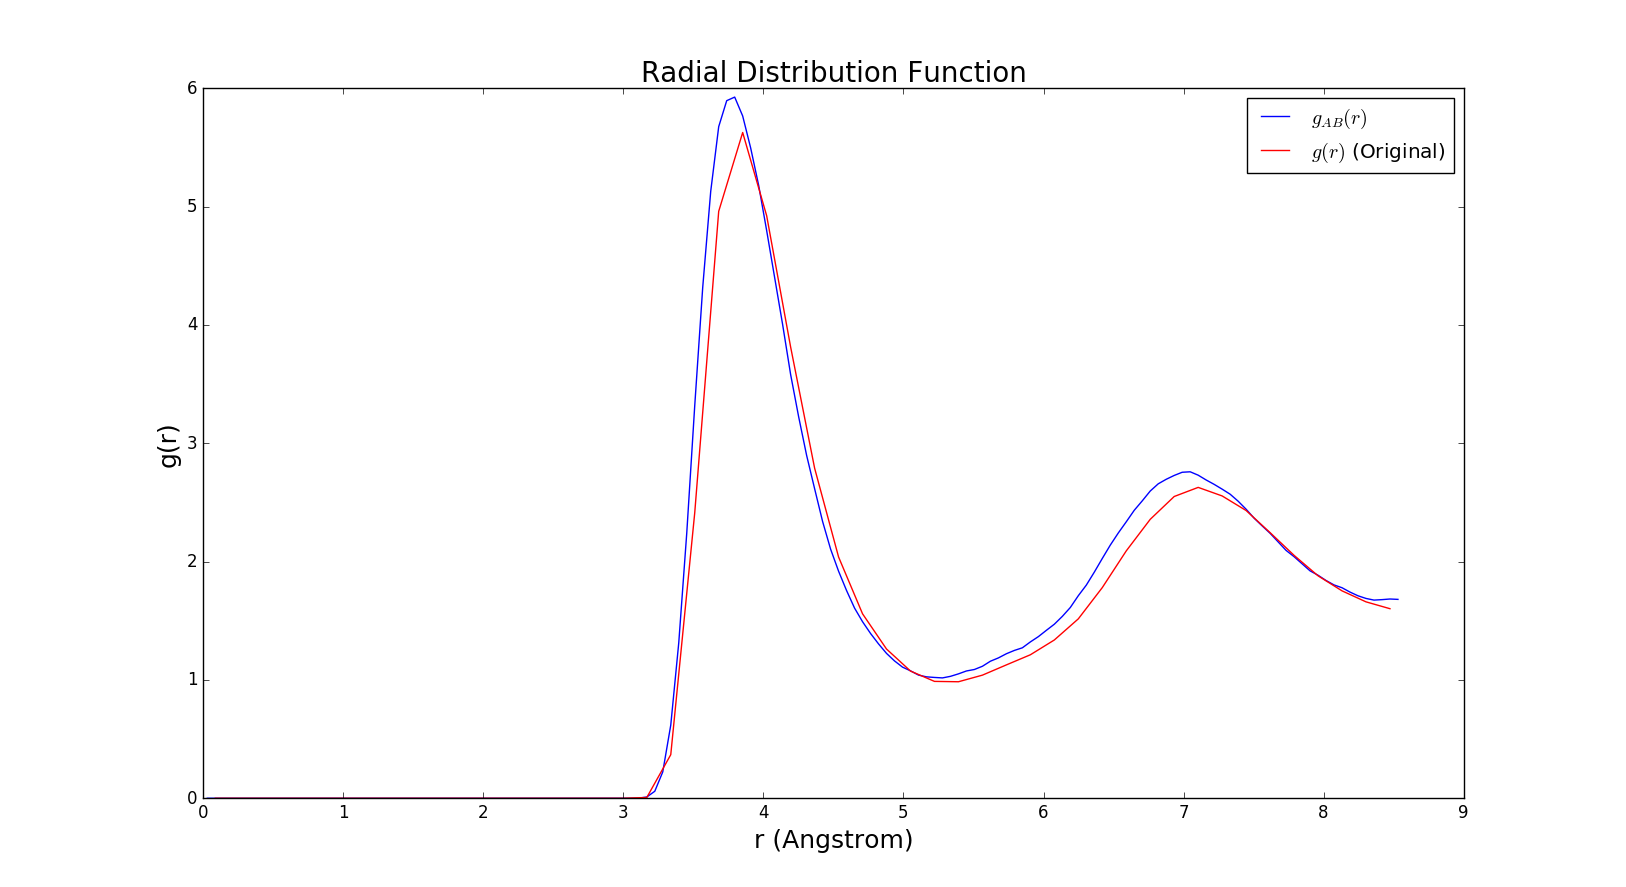
\includegraphics[scale=0.3]{../figures/PRDF_Q2.png}
    \caption{The partial radial distribution function is tested in the case when $A$ and $B$B are identical. \label{fig:PRDFTest}}
\end{figure}

Figure \ref{fig:PRDFTest} shows the result for the case in which species $A$ and $B$ are argon, compared with the radial distribution function generated from the original Pymold code. It can be seen that the partial distribution function generated follows closely to the RDF generated with the original pymold code.

\subsubsection{Self-Diffusion}

The normalised  velocity auto-correlation function is defined as 

\begin{equation}
C(t) = \frac{<v_i(t) \cdot v_i (0)>}{|v_i(t)||v_i(0)|}
\end{equation}

where $v_i(t)$ corresponds to the velocity of particle $i$ at time $t$. 

From this, the self-diffusion constant $D$ can be obtained through

\begin{equation}
\label{eqn:D1}
D = \frac{1}{3} \int_{0}^{\infty}C(t)dt.
\end{equation}

\begin{figure}[h]
    \centering
    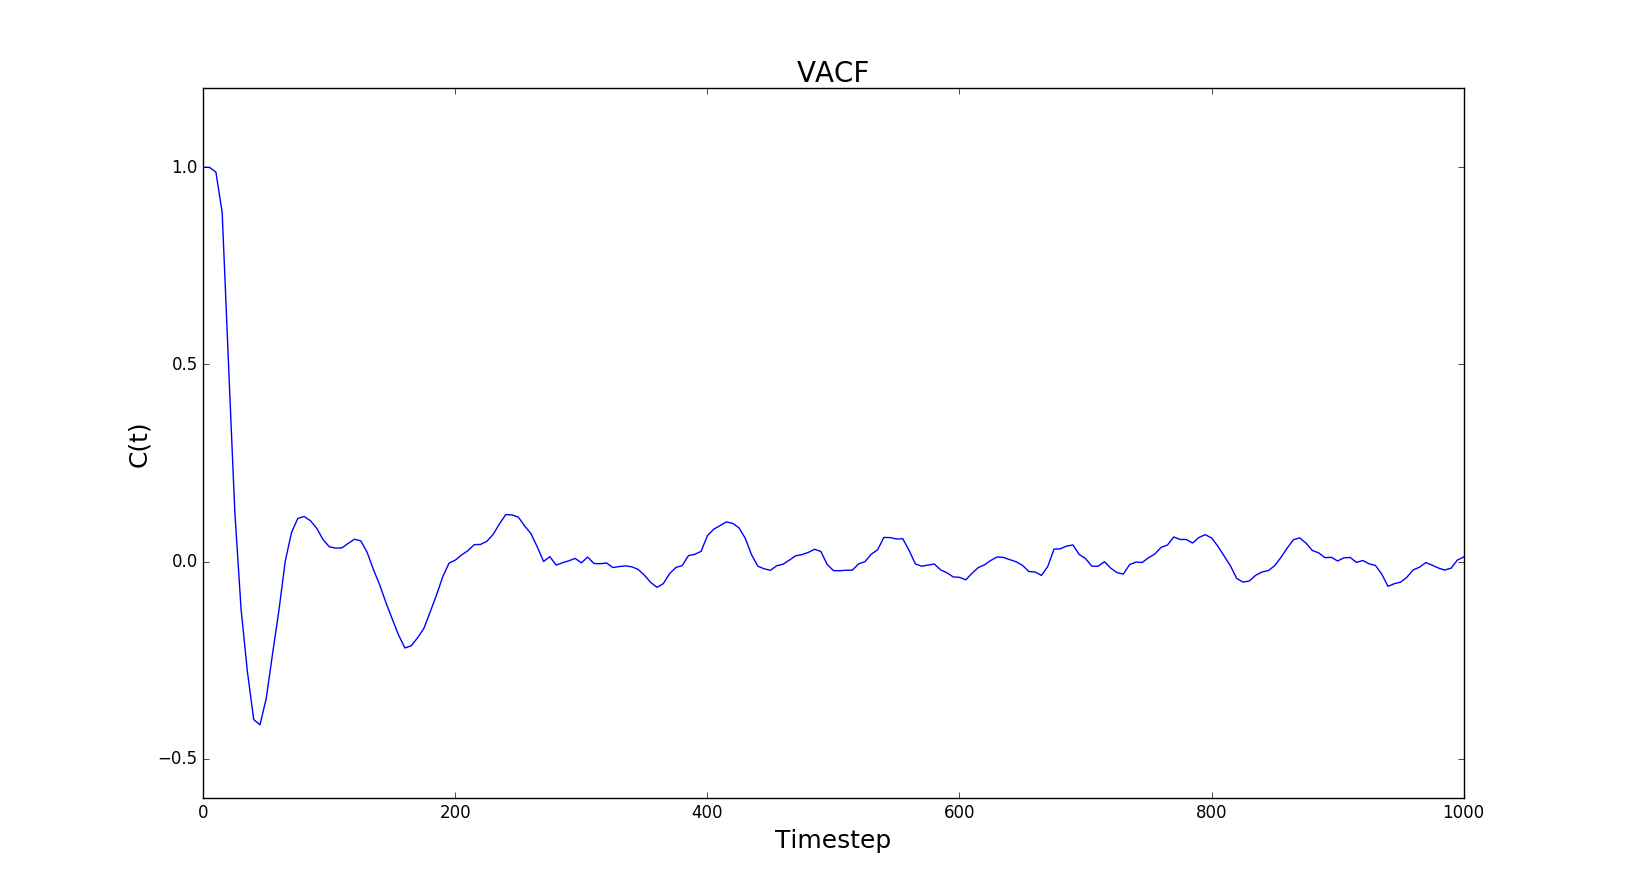
\includegraphics[scale=0.3]{../figures/VACF.png}
    \caption{The velocity autocorrelation function is plotted for argon. It can be seen that the VACF does not converge to zero. \label{fig:VACFTest}}
\end{figure}

However, from Figure \ref{fig:VACFTest} it can be seen that the velocity autocorrelation function does not tend towards zero as the number of time-steps increases, instead fluctuating randomly around zero. This is likely due to the finite number of particles in the system, with the . Therefore, \ref{eqn:D1} cannot be used to determine the self-diffusion coefficient, as summing the autocorrelation at each step will produce a `random walk' effect, causing the value for $D$ to diverge from the true value.

The self-diffusion constant can also be obtained through the relation 

\begin{equation}
\frac{\partial <r^2>}{\partial t} = 6D,
\end{equation}

where $<r^2>$ is the mean square displacement.

In \cite{StructureAndDiffusion}, the coefficient of mutual diffusion is expressed as

\begin{equation}
D_{12} = c_2 D_1 + c_1 D_2 + k_{\rm{B}}T\left( \frac{c_2}{m_1} + \frac{c_1}{m_2} \right)\int_{0}^{t}Q(t)dt,
\end{equation}

where $m_1$ and $m_2$ are the masses of the argon and krypton atoms respectively,and $Q(t)$ is the sum of the all cross-correlations of the velocities of different particles $<v_i(0)\cdot v_j(t)>$, where $i\neq j$.

This can be approximated by the equation

\begin{equation}
D_{12} \approx c_2 D_1 + c_1 D_2.
\end{equation}

\section{Results}

The partial radial distribution functions and self-diffusion coefficients were investigated for an argon-krypton mixture, using the same initial conditions as in \cite{StructureAndDiffusion}. The starting conditions involved an initial temperature of $115.8\,$K and a number density of $0.017614\,\rm{\r{A}}^{-3}$.
Given that there are 4 atoms in the primitive cell in the initial state of the system in pymold, this requires that the length of the primitive cell be $6.1010\,\rm{\r{A}}$.


\begin{table}[h!t]
\centering
\caption{ The results listed in \cite{StructureAndDiffusion} for a mixture of argon and krypton. From left to right: $c_1$, the fraction of particles in the mixture of type `1' (i.e. argon); $D_{12}$, the coefficient of mutual diffusion for the mixture at the given concentrations; $D_{1}$ and $D_2$, the extrapolated coefficients of self-diffusion for argon and krypton, respectively.}
\begin{tabular}{|c|c|c|c|} 
\hline
$c_1$ & $D_{12}$ & $D_1$ & $D_2$\\\hline
 & \multicolumn{3}{|c|}{($10^{-5}\,\rm{cm}^2\rm{s}^{-1}$)}\\\hline
$0.25$ & $2.3$ & $2.12$ & $1.79$\\
$0.5$ & $2.8$ & $3.01$ & $2.40$\\
$0.75$ & $3.0$ & $3.91$ & $3.25$\\\hline
\end{tabular}
\end{table} 


\bibliographystyle{unsrt}
\bibliography{./references}
\end{document}
